% Chapter 2

\chapter{Traducción de problemas NP}
\label{Chapter2}
\lhead{Capítulo 2. \emph{Traducción de problemas NP}}
Este capítulo describe el diseño de una herramienta capaz de transformar una
descripción de un problema en lógica de segundo orden existencial
en un problema de planificación perteneciente a la clase de complejidad
equivalente (NP).
Primero se explica el funcionamiento a alto nivel de la herramienta, en función
de sus entradas y salidas. Luego, se define formalmente una función de
traducción de lógica a planificación, demostrando las propiedades pertinentes.
Finalmente, se presenta la gramática de un lenguaje de especificación basado en lógica 
y se describe brevemente la implementación de la herramienta, que consiste en un 
analizador sintáctico para el lenguaje lógico encadenado con la función de traducción descrita.

\section{Perspectiva general}
Desde el punto de vista del usuario, la contribución de esta herramienta es
proveer una forma alternativa y descriptiva de especificar problemas de forma
que sea posible obtener e interpretar su solución.

Como puede verse en la Figura \ref{esquema_herramienta}, la herramienta tiene
como entradas una sentencia $\Phi\in\SOE(\sigma)$, y
una estructura finita de primer orden $\A\in\struc[\sigma]$ sobre la cual se
intentará probar la propiedad definida por $\Phi$.
Las salidas son un dominio y una instancia PDDL que tienen un plan válido si y
sólo si $\A$ satisface $\Phi$. Además, un \textbf{certificado} de la validez de
la propiedad en $\Phi$ puede obtenerse del plan en tiempo lineal.

\begin{figure}[h]
\centering
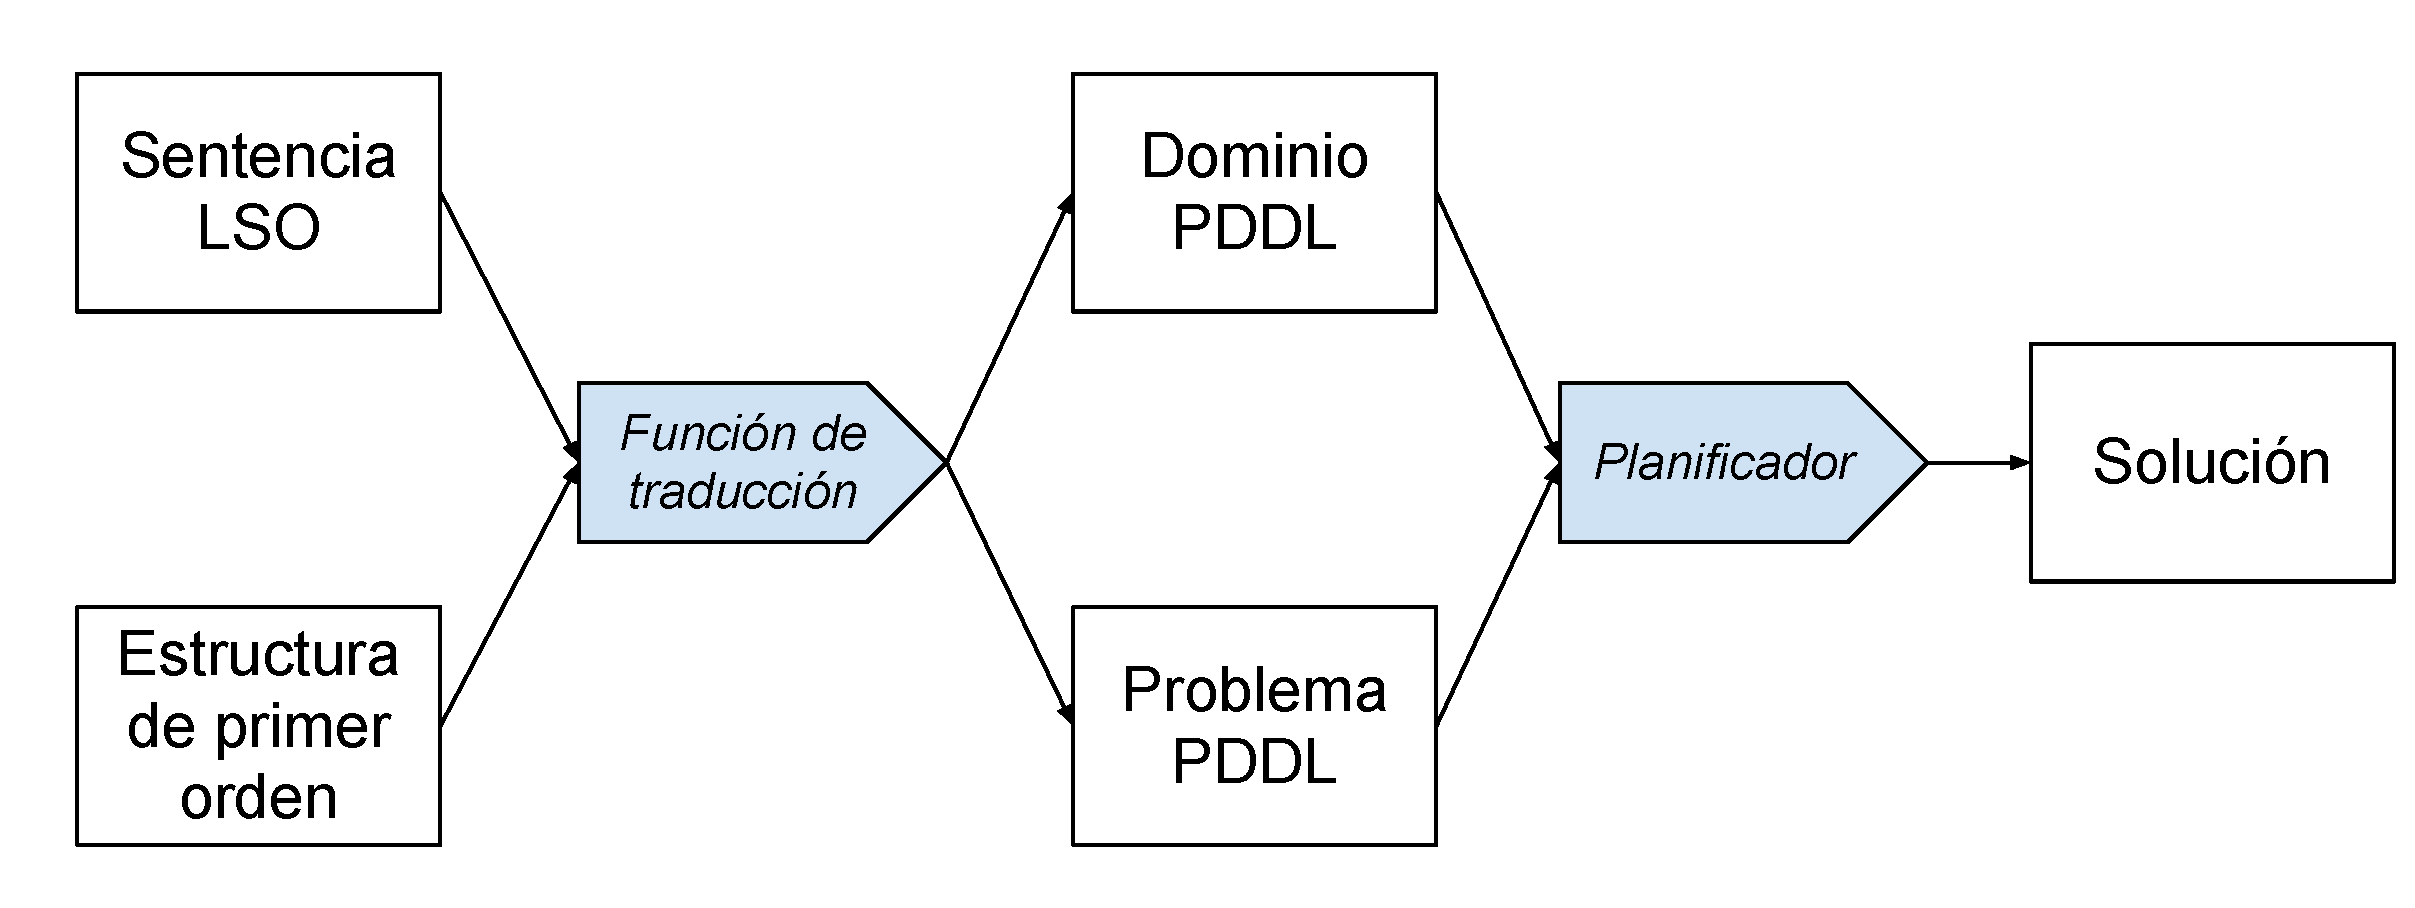
\includegraphics[width=\textwidth]{figuras/esquema_herramienta.pdf}
\caption{Esquema de operación de la herramienta}
\label{esquema_herramienta}
\end{figure}

La traducción se basa en convertir la tarea de demostrar la validez de la
fórmula lógica en una tarea de planificación. Por lo tanto, las acciones del
dominio de planificación hacen las veces de las definiciones de la semántica
formal, probando cada tipo de subfórmula según un esquema similar a la
definición \ref{semantica_def}. La información específica al problema, como el
estado inicial, está codificada por la estructura de primer orden que recibe la
herramienta. Se ha visto que estas estructuras pueden representar grafos, por lo
que el \textit{software} es especialmente útil para la modelación y resolución
de problemas de grafos.

\section{Reducción de LSO a STRIPS}
Una \textbf{reducción} de un problema $A$ a un problema $B$ es una función
computable $f$ tal que para cada instancia
$\omega$, $\omega\in A$ si y sólo si $f(\omega)\in B$.
La herramienta puede ser considerada un generador de reducciones entre problemas.

En este caso, la reducción se descompone en dos funciones
\begin{alignat*}{1}
&\domred: \text{Firmas} \times \SOE \rightarrow \text{Dominios PDDL}\,, \\
&\insred: \text{Firmas} \times \SOE \times \struc \rightarrow \text{Instancias PDDL}
\end{alignat*}
tal que $\domain=\domred(\sigma,\Phi)$ es un dominio PDDL
y $\instance=\insred(\sigma,\Phi,\A)$ es una instancia PDDL.

Para obtener algo de interés teórico y práctico, la reducción debe correr en
tiempo polinomial y su salida debe ser resoluble en NP para que la complejidad
de resolver su salida no sea mayor que la complejidad de resolver su entrada.

%Un problema STRIPS instanciado es una tupla $P=\tup{C,A,I,F}$
%donde $C$ es un conjunto de condiciones (proposiciones),
%$I\subseteq C$ denota el estado inicial,
%$F\subseteq C$ denota el estado final
%y $A$ es una colección de operadores.
%
%Each action $a\in O$ is defined by three subsets of fluents $pre(a)$,
%$add(a)$ and $del(a)$ that stand for the precondition, and the
%positive and negative effects of the action.
%As usual, action $a$ is applicable at state $s\subseteq F$ iff
%$pre(a)\subseteq s$, and the result of applying $a$ at such state
%is $res(s,a)=(s\setminus del(a))\cup add(a)$.
%A plan for state $s$ is a sequence of actions applicable from the
%initial state $I$ that achieves the goal condition.

%, and hence the \emph{grounding}
%of $\tup{\domain,\instance}$ results in an STRIPS problem $P$.
%The size of the grounding is polynomial for \emph{fixed} domain,
%but exponential for unrestricted domain and instance.

\subsection{Reducción del dominio}

$\domred(\sigma,\Phi)$ produce un dominio para la firma
$\sigma$ y la sentencia $\Phi\in\LSO(\sigma)$ de la forma
$(\exists R_1^{a_1})\cdots(\exists R_n^{a_n})\psi$.
Las acciones en el dominio se dividen en tres grupos: \textbf{acciones para 
colocar el valor de verdad de las variables de segundo orden} (relaciones
cuantificadas), \textbf{acciones para probar la sentencia} $\psi$ y \textbf{otras
acciones}.

\subsubsection{Acciones para las variables}
Para cada variable de segundo orden $R_i$ de aridad $a_i$,
existe una acción \fttt{colocar\_verdadera\_Ri} con $a_i$ parámetros que
coloca la condición \fttt{Ri} y quita $\fttt{libre-Ri}$, el cual debe ser
verdadero en el estado inicial de cualquier problema;
estas condiciones se usan para denotar el valor de
verdad de $R_i$. Por ejemplo, la acción para la relación $T^1$ en SAT es

{\footnotesize
\begin{Verbatim}
(:action colocar_verdadera_T
  :parameters (?x)
  :precondition (and (conjetura) (no-T ?x))
  :effect (and (T ?x) (no (no-T ?x))))
\end{Verbatim}
}

\subsubsection{Acciones para las subfórmulas}
Los operadores del segundo tipo están diseñados para construir una prueba de
$\psi$ (si existe) por inducción sobre la estructura de $\psi$.
Para cada subfórmula $\theta$ de $\psi$, hay una condición
$\FT[\theta]$ que denota su validez, y hay una acción que la añade.
Los parámetros de la condición $\FT[\theta]$ son las variables libres de
$\theta$; la función $\FT[\cdot]$ se llama la \textit{traducción de la
condición}.

El primer paso en la traducción es quitar todas las implicaciones
y mover todas las negaciones hacia los literales mediante aplicaciones
repetidas de las leyes de De~Morgan. Luego, se generan las acciones recorriendo
recursivamente todas las subfórmulas $\theta$ de $\psi$ utilizando
búsqueda en profundidad de la siguiente forma:
\footnote{$\theta(\bar x)$ significa que
$\bar x$ son las variables libres de $\theta$.}

\begin{enumerate}[--]
\item si $\theta(\bar x)=\bigwedge_{i=1}^n \theta_i(\bar x_i)$
  con $\bar x=\cup_{i=1}^n \bar x_i$, entonces generar la acción
  $\texttt{probar\_y}[\theta]$ con parámetros $\bar x$, precondición
  $\bigwedge_{i=1}^n \FT[\theta_i](\bar x_i)$ y efecto \textit{add}
  $\FT[\theta](\bar x)$,
%
\item si $\theta(\bar x)=\bigvee_{i=1}^n \theta_i(\bar x_i)$ con
  $\bar x=\cup_{i=1}^n \bar x_i$, entonces generar $n$ acciones de la forma
  $\texttt{probar\_o}[\theta]_i(\bar x_i)$ con precondición
  $\FT[\theta_i](\bar x_i)$ y efecto \textit{add} $\FT[\theta](\bar x)$,
%
\item si $\theta(\bar x)=(\exists y)\theta'(\bar x,y)$, entonces generar
  $\texttt{probar\_existencial}[\theta](\bar x,y)$ con precondición $\FT[\theta'](\bar x,y)$
  y efecto \textit{add} $\FT[\theta](\bar x)$,
%
\item si $\theta(\bar x)=(\forall y)\theta'(\bar x,y)$ entonces generar
  dos acciones. La idea es probar $\theta(\bar x)$, variando $y$
  sobre todos los objetos.

  La primera acción $\texttt{probar\_universal\_base}[\theta](\bar x)$ prueba $\theta'(\bar x,0)$.
  La acción tiene parámetros $\bar x$, precondición $\FT[\theta'](\bar x,0)$
  y efecto \textit{add} $\FT[(\forall y\leq z)\theta'(\bar x,y)](\bar x,0)$.
  (Observar que la traducción de la condición es aplicada a diferentes
fórmulas,
  en las cuales la cuantificación está acotada por $z$.)

  La segunda acción $\texttt{probar\_universal\_inductivo}[\theta]_1(\bar x,z',z'')$ prueba inductivamente
  $(\forall y\leq z)\theta'(x,y)$ una vez que $(\forall y<z)\theta'(x,y)$ es
verdad.
  La acción tiene parámetros $\bar x,z',z''$, precondición
  $\FT[(\forall y\leq z)\theta'(\bar x, y)](\bar x,z')\land\FT[\theta'](\bar x,z'')\land \SUC(z',z'')$
  y efecto \textit{add} $\FT[(\forall y\leq z)\theta'(\bar x,y)](\bar x,z')$.
\end{enumerate}
Todas estas acciones tienen como precondición adicional la condición
\fttt{prueba}. Además, nótese que no hay acciones para las fórmulas literales.
Éstas son manejadas por la traducción de condiciones, cuya función es asignar
fórmulas a condiciones de esta manera:
\begin{enumerate}[--]
\item $\FT[Q(\bar x)](\bar x)=Q(\bar x)$,
\item $\FT[\neg Q(\bar x)](\bar x)=\fttt{no-}Q(\bar x)$,
\item $\FT[(\forall y)\theta'(\bar x,y)](\bar x) =
  \FT[(\forall y\leq z)\theta'(\bar x,y)](\bar x,\max)$,
\item en cualquier otro caso, $\FT[\theta](\bar x)=\fttt{es\_cierto\_<id>}(\bar x)$
  donde \fttt{<id>} es un identificador único para $\theta$.
\end{enumerate}
La función de traducción también se encarga de instanciar variables a términos
cuando es aplicada a literales que involucran a constantes.

\subsubsection{Otras acciones}
La traducción requiere de dos otras acciones. La primera,
llamada \fttt{empezar\_prueba} sirve para cambiar la fase de
`conjetura' a `prueba', tiene precondición \fttt{conjetura}, agrega
\fttt{prueba} y quita \fttt{conjetura}. La otra acción se llama
\fttt{probar-meta}, tiene precondición $\FT[\psi]$ y agrega 
\fttt{es\_cierto\_meta}.

%Figure~\ref{figure:sat} shows the domain for $\Phi_\SAT$.

%\begin{SaveVerbatim}{SAT}
%(define (domain SAT)
%  (:constants zero max)
%  (:predicates
%    (holds_and_2 ?x ?y) (holds_and_6 ?x0 ?x1)
%    (holds_exists_8 ?x0) (holds_forall_9 ?x0)
%    (holds_or_7 ?x0 ?x1) (holds_goal)
%    (N ?x ?y) (P ?x ?y) (T ?x) (not-T ?x)
%    (suc ?x ?y)
%  )
%  (:action set_T_true
%    :parameters (?x)
%    :precondition (and (guess) (not-T ?x))
%    :effect (and (T ?x) (not (not-T ?x))))
%
%  (:action prove_forall_9_1
%    :precondition (and (proof)
%                       (holds_exists_8 zero))
%    :effect (holds_forall_9 zero))
%
%  (:action prove_forall_9_2
%    :parameters (?y1 ?y2)
%    :precondition (and (proof)
%                       (suc ?y1 ?y2)
%                       (holds_forall_9 ?y1)
%                       (holds_exists_8 ?y2))
%    :effect (holds_forall_9 ?y2))
%
%  (:action prove_exists_8
%    :parameters (?y ?x)
%    :precondition (and (proof)
%                       (holds_or_7 ?y ?x))
%    :effect (holds_exists_8 ?y))
%
%  (:action prove_or_7_0
%    :parameters (?y ?x)
%    :precondition (and (proof)
%                       (holds_and_2 ?y ?x))
%    :effect (holds_or_7 ?y ?x))
%
%  (:action prove_or_7_1
%    :parameters (?y ?x)
%    :precondition (and (proof)
%                       (holds_and_6 ?y ?x))
%    :effect (holds_or_7 ?y ?x))
%
%  (:action prove_and_2
%    :parameters (?y ?x)
%    :precondition (and (proof)
%                       (P ?x ?y) (T ?x))
%    :effect (holds_and_2 ?y ?x))
%
%  (:action prove_and_6
%    :parameters (?y ?x)
%    :precondition (and (proof)
%                       (N ?x ?y) (not-T ?x))
%    :effect (holds_and_6 ?y ?x))
%
%  (:action prove-goal
%    :precondition (holds_forall_9 max)
%    :effect (holds_goal))
%
%  (:action begin-proof
%    :precondition (guess)
%    :effect (and (proof) (not (guess)))) )
%\end{SaveVerbatim}

%\begin{figure}
%\begin{center}
%\footnotesize
%\UseVerbatim{SAT}
%\end{center}
%\vskip -.85em
%\caption{Domain translation for $\Phi_\text{sat}=(\exists T^1)(\forall y)(\exists x)$
%$[(P(x,y)\land T(x))\lor(N(x,y)\land\neg T(x))]$.}
%\label{figure:sat}
%\end{figure}

\subsubsection{Abreviaciones}
Al haber abreviaciones, las acciones para las variables de segundo orden son
extendidos para hacer la traducción más eficiente. Para $(\exists F\in\Fun)$,
la precondición y el \textit{delete} de \fttt{colocar\_verdadera\_F} son
extendidos con la condición \fttt{(libre\_F\_dom ?x)} de modo de que pueda
haber a lo sumo una condición $F(x,y)$ verdadera para cada $x$. Así, no hay
necesidad de incluir la subfórmula $\psi_\text{fun}$. 

De forma similar, para $(\exists F\in\Inj)$ la precondición y el
\textit{delete}
son extendidos adicionalmente con la condición \fttt{(libre\_F\_ran ?y)}.

\subsection{Problema}

\label{traduccionproblema}
El problema PDDL es generado por la llamada $\insred(\sigma,\Phi,\A)$, donde
$\sigma$ es una firma, $\Phi\in\LSO(\sigma)$ y $\A\in\struc[\sigma]$.
Los objetos en el problema corresponden a los elementos en el universo
$|\A|=\{0,\ldots,n-1\}$: $0$ se asigna al objeto
\fttt{zero}, $n-1$ al objeto \fttt{max}, y los otros elementos
$0<i<n-1$ a los objetos \fttt{obj\_i}.
El objetivo es alcanzar la condición \fttt{es\_cierto\_meta}, y la situación
inicial consiste en condiciones describiendo el valor de verdad de todas las
relaciones en $\A$ y las relaciones predefinidas como $<$, SUC y otras. Sin
embargo, no es necesario incluir condiciones para relaciones que no se
mencionan en $\Phi$. Además, para cada variable de segundo orden $R$, la
situación inicial tiene condiciones que denotan que los valores de verdad de
$R$ no han sido asignados (\fttt{libre\_f}), y en casos en los que un símbolo
represente una función o función inyectiva, la situación inicial incluye
condiciones del tipo \fttt{libre\_R\_dom} y \fttt{libre\_R\_ran}.


\section{Propiedades formales}
Las propiedades más importantes a considerar en la herramienta son solidez,
completitud y garantía de complejidad. Que la función de traducción sea sólida
y completa significa que ella realmente implementa una reducción entre problemas de
decisión, mientras que la garantía de complejidad se refiere al tiempo
requerido para computar la reducción y a la complejidad de decidir la existencia
de un plan en el problema generado.

Recuerde que la reducción se descompone en dos funciones $\domred :
\text{Firmas} \times \SOE \rightarrow \text{Dominios PDDL}$, y $\insred :
\text{Firmas} \times \SOE \times \struc \rightarrow \text{Instancias PDDL}$,
tal que $\domain=\domred(\sigma,\Phi)$ es un dominio PDDL
y $\instance=\insred(\sigma,\Phi,\A)$ es una instancia PDDL.

Considere la función de \emph{instanciación} $\ground$ que transforma el par
$\tup{\domain,\instance}$ de un dominio y problema PDDL en un problema STRIPS
$P = \ground(\domain, \instance)$.

Formalmente, $f_{\sigma,\Phi}:\struc[\sigma]\rightarrow\text{STRIPS}$
definida por 
\[ f_{\sigma,\Phi}(\A) = \ground(\domred(\sigma,\Phi),\insred(\sigma,\Phi,\A)) \]
es una función que asigna a las $\sigma$-estructuras un
problema instanciado STRIPS.

A continuación se demuestran las tres propiedades formales importantes sobre
$f_{\sigma,\Phi}$.

\subsection{Demostración de reducción}
Se demostrará que $\A \models \Phi$ si y sólo si $f_{\sigma,\Phi}(\A)$ tiene
solución, es decir, si y sólo si existe un plan que alcanza $\FT[\Phi]$ desde
el estado inicial (que depende de $\A$).

\begin{proposition}
\label{t1}
Sean $t_1,\ldots,t_k$ términos instanciados, es decir, que no contienen
variables. Sea $\A$ una estructura, $u\in|\A|$ y `$a$' una constante tal que
$a^\A=u$.
Entonces, $(\A, i[x:=u]) \models \varphi(t_1,\ldots,t_k,x)$ si y sólo si
$(\A, i) \models \varphi(t_1,\ldots,t_k,a)$.
\end{proposition}
\begin{proof}
Directa de la definición de verdad.
\end{proof}
\begin{corollary}
\label{corolario}
Sean $t_1,\ldots,t_k$ términos instanciados. Sea $\A$ una
estructura en donde todos los objetos tienen nombre (i.e., para todo $u\in|\A|$
existe una constante $a$ tal que $a^\A=u$). Entonces,
$(\A, i) \models (\exists x) \varphi(t_1,\ldots,t_k,x)$ si y sólo si
existe una constante `$a$' tal que $(\A, i) \models \varphi(t_1,\ldots,t_k,a)$.
\end{corollary}

\begin{theorem}
\label{teoremaprimerorden}
Sea $\varphi \in \LPO(\sigma)$ y $t_1,\ldots,t_k$ $\sigma$-términos instanciados. Sea $\A \in
\struc[\sigma]$ tal que todo objeto tiene nombre y sea $i : \text{VAR} \rightarrow |\A|$.
Entonces, $(\A, i) \models \varphi(t_1,\ldots,t_k)$ si y sólo si
existe un plan $\pi[t_1,\ldots,t_k]$ que alcanza
$\FT[\varphi](t_1,\ldots,t_k)$ desde el \textbf{estado intermedio} $I[\A]$,
el estado de STRIPS en el cual los operadores que construyen la
prueba empiezan a ser aplicables, definido por las siguientes condiciones:
\begin{alignat*}{1}
& I[\A] = \{\texttt{prueba}\} \cup \{ \texttt{R}(a_1,\ldots,a_k) :
\tup{a_1^\A,\ldots,a_k^\A} \in R^\A\}\\
& {\color{white} I[\A] = } \cup \{\texttt{no-R}(a_1,\ldots,a_k) : \tup{a_1^\A,\ldots,a_k^\A} \not\in R^\A\}\\
& {\color{white} I[\A] = } \cup \{\texttt{SUC}(a_i, a_{i+1}) : 0 \leq i < n\}
\end{alignat*}
\end{theorem}
\begin{proof}
Hacemos la demostración por inducción sobre la estructura de $\varphi$. El caso
base corresponde a las fórmulas atómicas de la forma $\varphi =
R(t_1,\ldots,t_k)$:
\begin{alignat*}{1}
& \quad \quad (\A, i) \models \varphi(t_1,\ldots,t_k)\\
& \iff \tup{\text{definición \ref{semantica_def}(b)}} \\
& \quad \quad \tup{t_1,\ldots,t_k} \in R^\A\\
& \iff \tup{\text{definición de I[\A]}}\\
& \quad \quad \texttt{R}(t_1,\ldots,t_k) \in I[\A]\\
& \iff \tup{\text{definición de } \FT}\\
& \quad \quad \FT[\varphi](t_1,\ldots,t_k) \in I[\A]\\
& \iff \tup{\text{el plan vacío alcanza la condición } \FT[\varphi](t_1,\ldots,t_k)}\\
& \quad \quad \pi[t_1,\ldots,t_k] =\ \tup{} \textbf{ es el plan.}
\end{alignat*}
El caso $\varphi = \neg R(t_1,\ldots,t_k)$ es análogo al anterior, con
\texttt{not-R}$(t_1,\ldots,t_k) \in I[\A]$ en lugar de \texttt{R}$(t_1,\ldots,t_k)$.
Ahora consideramos las fórmulas más complejas:

Caso $\varphi = \varphi_1(t'_1,\ldots,t'_{k'}) \land \varphi_2(t_1'',\ldots,t''_{k''}) $:
\begin{alignat*}{1}
& \quad \quad (\A, i) \models \varphi(t_1,\ldots,t_k)\\
& \iff \tup{\text{definición \ref{semantica_def}(d)}}\\
& \quad \quad (\A, i) \models \varphi_1(t'_1,\ldots,t'_{k'}) \text{ y } 
(\A, i) \models \varphi_2(t''_1,\ldots,t''_{k''})\\
& \iff \tup{\text{hipótesis inductiva}}\\
& \quad \quad \pi_1[t'_1,\ldots,t'_{k'}] \text{ y } 
\pi_2[t_1'',\ldots,t''_{k''}] \text{ son planes que alcanzan }\\
& \quad \quad \FT[\varphi_1](t'_1,\ldots,t'_{k'}) \text{ y } \FT[\varphi_2](t'_1,\ldots,t'_{k''})
\text{ desde } I[\A]\\
& \iff \langle \text{como no hay \textit{deletes}, aplicar ambos planes en
secuencia }\\
& {\color{white}\iff\langle} \text{garantiza alcanzar
$\FT[\varphi](t_1,\ldots,t_k)$ desde $I[\A]$} \rangle\\
& \quad \quad \textbf{el plan }\tup{\pi_1(t'_1,\ldots,t'_{k'});\
\pi_2(t_1'',\ldots,t_{k_2}'');\ \texttt{probar\_y\_}\varphi(t_1,\ldots,t_k)} \\
& \quad \quad \textbf{alcanza la condición }
\FT[\varphi](t_1,\ldots,t_k) \textbf{ desde } I[\A]
\end{alignat*}

Caso $\varphi = \varphi_1(t_1',\ldots,t'_{k_1}) \lor \varphi_2(t''_1,\ldots,t''_{k_2}) $:
\begin{alignat*}{1}
& \quad \quad (\A, i) \models \varphi(t_1,\ldots,t_k)\\
& \iff \tup{\text{definición \ref{semantica_def}(e)}}\\
& \quad \quad (\A, i) \models \varphi_1(t'_1,\ldots,t'_{k'}) 
\text{ o } (\A, i) \models \varphi_2(t''_1,\ldots,t''_{k''})\\
& \text{Por casos. Caso $(\A, i) \models \varphi_1(t'_1,\ldots,t'_{k'})$:}\\
& \quad \iff \tup{\text{hipótesis inductiva}}\\
& \quad \quad \quad \pi_1[t_1,\ldots,t_{k_1}] \text{ es un plan que alcanza 
$\FT[\varphi_1](t_1,\ldots,t_{k_1})$ desde $[\A]$}\\
& \quad \iff \langle \text{no hay \textit{deletes}} \rangle\\
& \quad \quad \textbf{el plan } \tup{\pi_1(t_1,\ldots,t_{k_1});\
\texttt{probar\_o\_}\varphi(t_1,\ldots,t_k)} \\
& \quad \quad \textbf{alcanza la condición }
\FT[\varphi](t_1,\ldots,t_k) \textbf{ desde } I[\A]\\
& \text{Caso $(\A, i) \models \varphi_2(t''_1,\ldots,t''_{k''})$:}\\
& \quad \quad \text{Análogo al caso anterior.}
%Caso $\varphi = \varphi_1(t_1',\ldots,t'_{k'}) \Rightarrow \varphi_2(t''_1,\ldots,t''_{k''}) $:
%\quad Ver caso anterior, pues $\varphi_1 \Rightarrow \varphi_2 = \neg \varphi_1 \lor \varphi_2$.
\end{alignat*}

Caso $\varphi = (\exists x)\ \theta(t_1,\ldots,t_k,x):$
\begin{alignat*}{1}
& \quad \quad (\A, i) \models \varphi\\
& \iff \langle \text{por corolario \ref{corolario}, ya que todo objeto en $|\A|$
tiene nombre, }\\
& {\color{white} \iff \langle} \text{ existe una constante } `a' \rangle\\
& \quad \quad (\A, i) \models \theta(t_1,\ldots,t_k,a)\\
& \iff \tup{\text{hipótesis inductiva}}\\
& \quad \quad \pi[t_1,\ldots,t_k,a] \text{ es un plan que alcanza }
\FT[\theta](t_1,\ldots,t_k,a) \text{ desde } I[\A]\\
& \iff \tup{\text{no hay \textit{deletes}}}\\
& \quad \quad \textbf{el plan } \langle \pi[t_1,\ldots,t_k,a];\
\texttt{probar\_existencial\_}\varphi(t_1,\ldots,t_k)\rangle\\
& \quad \quad \textbf{alcanza la condición } \FT[\varphi](t_1,\ldots,t_k)
\textbf{ desde } I[\A]
\end{alignat*}

Caso $\varphi = (\forall x)\ \theta(t_1,\ldots,t_k,x):$
\begin{alignat*}{1}
& \quad \quad (\A, i) \models \varphi\\
& \iff \tup{\text{definición \ref{semantica_def}(h), y todo objeto tiene nombre}}\\
& \quad \quad (\A, i) \models \theta(t_1,\ldots,t_k,a), \text{ para toda
constante $a$}\\
& \iff \tup{\text{hipótesis inductiva}}\\
& \quad\quad \text{para toda constante $a$ existe un plan $\pi[t_1,\ldots,t_k,a]$ que}\\
& \quad\quad \text{alcanza $\FT[\theta](t_1,\ldots,t_k,a)$ desde } I[\A]\\
& \iff \langle \text{existe un orden $a_i < a_{i+1}$ para todas las constantes,}\\
& {\color{white} \iff \langle} \text{ determinado por \texttt{SUC}, y no hay
\textit{deletes}} \rangle\\
& \quad \quad \textbf{el plan } \langle \pi_0[t_1,\ldots,t_k,a_0];\
\texttt{probar\_universal\_base\_}\varphi(t_1,\ldots,t_k,a_0);\\
& \quad \quad \pi_1[t_1,\ldots,t_k,a_1];\
\texttt{probar\_universal\_inductivo\_}\varphi(t_1,\ldots,t_k,a_0,a_1);\\
& \quad \quad \ldots\ \\
& \quad \quad \pi_{n-1}[t_1,\ldots,t_k,a_{n-2},a_{n-1}];\
\texttt{probar\_universal\_inductivo\_}\varphi(t_1,\ldots,t_k,a_{n-2},a_{n-1}) \rangle\\
& \quad \quad \textbf{alcanza la condición } \FT[\varphi](t_1,\ldots,t_k)
\textbf{ desde } I[\A]
\end{alignat*}
\end{proof}

\begin{definition}
Sea $\Phi = (\exists R_1^{k_1})\cdots(\exists R_m^{k_m}) \varphi$.
El \textbf{estado inicial} \textsc{init}[\A] de un problema STRIPS generado por
$f_{\sigma,\Phi}(\A)$ es:
\begin{alignat*}{1}
& \textsc{init}(\A) = \{\{ \texttt{P}(a_1,\ldots,a_k) :
\tup{a_1^\A,\ldots,a_k^\A} \in P^\A\}\\
& {\color{white} \texttt{init}[\A] = } \cup \{\texttt{no-P}(a_1,\ldots,a_k) : \tup{a_1^\A,\ldots,a_k^\A} \not\in P^\A\}\\
& {\color{white} \texttt{init}[\A] = } \cup \{\texttt{SUC}(a_i, a_{i+1}) : 0 \leq i < n \} \\
& {\color{white} \texttt{init}[\A] = } \cup \{\texttt{libre-R\_i}(t)) : \text{ para todo $t \in |\A|^{k_i}$},
R_i\in\{R_1,\ldots,R_m\}\} \}
\end{alignat*}
\end{definition}

Finalmente, puede probarse que la función es una reducción:
\begin{theorem}
Sea $\Phi = (\exists R_1)\cdots(\exists R_n) \varphi$.
$\A \models \Phi$ si y sólo si existe un plan $\pi$ que alcanza $\FT[\Phi]$
desde el estado inicial $\textsc{init}(f_{\sigma,\Phi}(\A))$.
\end{theorem}
\begin{proof}
Por definición, $\A \models \Phi$ si y sólo si
$\tup{\A, R_1',\ldots,R_n'} \models \varphi$.
Por Teorema \ref{teoremaprimerorden}, esto es verdad si y sólo si 
existe un plan $\pi'$ que alcanza $\FT[\varphi]$ a partir de $I[\A,
R_1',\ldots,R_n']$.
Basta mostrar que es posible alcanzar el estado $I[\A, R_1',\ldots,R_n']$ desde
$\textsc{init}(f_{\sigma,\Phi}(\A))$. Sea $u_j = a_j^\A$ para $1 \leq j \leq k$.
\begin{alignat*}{1}
& \textbf{El plan }\\
& \langle \ \tup{\texttt{colocar\_verdadera\_Ri}(a_1,\ldots,a_{k_i}) 
\text{ para cada } \tup{u_1,\ldots,u_k} \in R_i} \text{ para cada } R_i \ ;\\
& {\color{white} \langle \ } \tup{\texttt{colocar\_falsa\_Ri}(a_1,\ldots,a_{k_i}) \text { para cada
} \tup{u_1,\ldots,u_k} \not\in R_i} \text{ para cada } R_i\ ;\\
& {\color{white} \langle \ } \texttt{comenzar\_prueba}()\ \rangle\\
& \textbf{alcanza el estado } I[\A, R_1',\ldots,R_n'] \textbf{ desde }
\textsc{init}(f_{\sigma,\Phi}(\A)).
\end{alignat*}
\end{proof}

\subsection{Tiempo de corrida de la reducción}
En esta sección se demuestra que $f_{\sigma,\Phi}$ es una reducción en tiempo
polinomial del problema NP expresado por $\Phi$ en STRIPS.

Recuerde que 
$ f_{\sigma,\Phi}(\A) = \ground(\domred(\sigma,\Phi),\insred(\sigma,\Phi,\A))
$.
Para un $\domain$ fijo, la función
$\instance\leadsto\ground(\domain, \instance)$ corre en un tiempo polinomial
$\O(\|\instance\|^k)$ para algún $k$ que sólo depende de $\domain$; de hecho,
$k$ es la máxima aridad de un predicado o acción en el dominio. Nótese que en
este caso el dominio puede generarse de manera independiente del problema 
utilizando sólo una fórmula de segundo orden. Al no depender de $\A$, el
dominio es fijo y $\domred$ corre en tiempo polinomial.

La función de traducción $\insred$ corre en tiempo
polinomial en el tamaño de la estructura $\A$, puesto que sólo se agregan
condiciones que equivalen al estado de las relaciones $P\in\sigma$ al estado inicial.

%pero exponencial sobre la aridad
%más grande de un cuantificador de segundo orden existencial en $\Phi$. 

\subsection{Complejidad de los problemas generados}
Se debe demostrar que los problemas de planificación producidos 
por $f_{\sigma,\Phi}(\A)$ tienen a lo sumo la misma
complejidad que \SOE.

El problema de decisión de existencia de un plan general para un problema
STRIPS no está en NP porque (1)~el número de condiciones y acciones instanciadas puede ser
exponencial en el tamaño de la entrada, y (2)~incluso los planes más cortos pueden
ser de tamaño exponencial en el número de condiciones y acciones instanciadas.
%Por lo tanto, no todas las reducciones son adecuadas para este propósito y su
%diseño debe realizarse cuidadosamente. En esta sección se
%presenta una reducción aceptable y se estudian sus propiedades formales.

Como se ha mencionado en la sección \ref{complejidad_planificacion}, 
se sabe que verificar la existencia de un plan para 
problemas de planificación
sin efectos negativos está en NP \citep{bylander:plan-complexity}. La prueba
depende del hecho de que un plan óptimo no necesita repetir acciones, y por lo
tanto es de tamaño lineal. Puede extenderse esta noción: si todas las acciones que
agregan efectos negativos pueden ser aplicadas a lo sumo una vez, verificar la
existencia de un plan sigue estando en NP, pues el tamaño del plan no podrá ser
mayor al número de acciones.

\begin{definition}
Un problema de planificación $P = \tup{C, A, I, F}$ es de tipo
\textit{máximo-1} si y sólo si las acciones pueden ser particionadas en $A =
A_0 \cup A_1$, donde:
\begin{itemize}
\item Ninguna de las acciones de $A_0$ tiene efectos negativos, es decir,
$(\forall a \in A_0) (del(a) = \emptyset)$.
\item Todas las acciones de $A_1$ tienen una precondición que no es añadida por
ninguna acción, y que es borrada apenas $a$ es ejecutada, es decir, 
$(\forall aa' \in A_1)\ (\exists p \in pre(a) \cap del(a))\ (p \not\in add(a'))$
\end{itemize}

El conjunto de todos los problemas \textit{máximo-1} se denota como STRIPS-1.
\end{definition}

\begin{theorem}
Para toda estructura $\A$, $f_{\sigma, \Phi}(\A)$ es un problema STRIPS-1.
\end{theorem}
\begin{proof}
Ninguna de las acciones de $f_{\sigma, \Phi}(\A)$ tienen \textit{deletes} excepto
\texttt{comenzar\_prueba} y las acciones \texttt{colocar\_verdadera} y
\texttt{colocar\_falsa}, pero todas estas borran una precondición que no es
añadida por ninguna otra acción (i.e., pertenecen a $A_1$ según la definición
de STRIPS-1).
\end{proof}

\begin{theorem}
El problema de decisión de existencia de un plan STRIPS-1 es NP-completo.
\end{theorem}
\begin{proof}
\ \\ \textbf{Inclusión:} Todas las acciones de $A_1$ pueden ser aplicadas a lo
sumo una vez. Como estas acciones pueden borrar condiciones (tienen
\textit{deletes}), en el peor caso puede requerirse aplicar \textbf{todas} las
acciones de $A_0$ antes de aplicar otra acción de $A_1$. Por lo tanto, el
tamaño de un plan es a lo sumo cuadrático en el número total de acciones.
\\ \textbf{Dificultad:} $f_{\sigma_{\textsc{SAT}}, \Phi_{\textsc{SAT}}}$ reduce SAT a STRIPS-1 en
tiempo polinomial.
\end{proof}

Por lo tanto, la herramienta traduce cualquier problema NP, codificado con una
sentencia \SOE, a un problema STRIPS-1 que se ubica en la clase de complejidad
NP.

\section{Diseño del lenguaje}
El lenguaje de entrada de la herramienta debe ser capaz de expresar
sintácticamente cualquier fórmula \LSO existencial. En el capítulo
\ref{Chapter4} se presenta una extensión de la herramienta que le permite
traducir problemas en la clase más compleja PH, por lo que es necesario
agregarle al lenguaje el operador $\forall$ de segundo orden, $\SOForall$.
La figura \ref{gramatica} muestra la gramática del lenguaje propuesto
en forma Backus-Naur, que permite especificar fórmulas lógicas generales de
segundo orden.

\begin{figure}[h]
\begin{alignat*}{1}
\sofbf\   & \deriv\ \lpar \SOExists\ \lpar \listrel \rpar\ \sofbf \rpar \\
          & \deriv\ \lpar \SOForall\ \lpar \listrel \rpar\ \sofbf \rpar \\
          & \deriv\ \pofbf \\[1em]
\listrel\ & \deriv\ \rel\ \integer\ \listrel\ |\ \rel\ \integer \\
          & \deriv\ \rel\ \tipof\ \listrel\ |\ \rel\ \tipof\ \\[1em]
\tipof\   & \deriv\ \Fun\ |\ \PFun\ |\ \Inj\ |\ \PInj\ \\[1em]
\pofbf\   & \deriv\ \lpar \rel\ \listvar \rpar \\
          & \deriv\ \lpar \NOT\ \pofbf \rpar \\
          & \deriv\ \lpar \AND\ \listpofbf \rpar \\
          & \deriv\ \lpar \OR\ \listpofbf \rpar \\
          & \deriv\ \lpar \IMPLIES\ \pofbf\ \pofbf \rpar \\
          & \deriv\ \lpar \Exists\ \lpar \listvar \rpar\ \pofbf \rpar \\
          & \deriv\ \lpar \Forall\ \lpar \listvar \rpar\ \pofbf \rpar \\[1em]
\listvar\ & \deriv\ \var\ \listvar\ |\ \var \\[1em]
\end{alignat*}
\label{gramatica}
\caption{Gramática en BNF del lenguaje que se utiliza para expresar $\Phi$ en
la herramienta.}
\end{figure}

Para especificar una firma $\sigma = \tup{R_1^{k_1},\ldots,R_n^{k_n}}$ se utiliza la notación:
\begin{verbatim}
?R_1 k_1
...
?R_n k_n
\end{verbatim}

Para especificar constantes en la firma se utilizan relaciones unarias que son
ciertas sólo para el elemento de $|\A|$ que interpreta la constante.
Esto simplifica el procesamiento. Por ejemplo, si se quiere agregar una
constante $K$ se agrega una relación unaria a la
firma \texttt{?K 1}.

%\subsubsection{Constantes}
%Los símbolos de constantes que pertenecen a la firma (por ejemplo,
%$K\in\sigma$) son `preprocesados' y convertidos a relaciones unarias
%que son ciertas para el elemento en $\A$ que interpreta $K$, i.e. $K^\A$.
%El preprocesamiento consiste en reescribir la 

%$K^\A$. The preprocessing consists of rewriting the logical %!fix
%formulae that use the constant into appropriate formulae that
%use the new relation, and in extending the initial situation of
%the problem with the value of the relation.

\section{Implementación de la herramienta}
La herramienta fue implementada en el lenguaje de programación \textit{python}.

El \textit{software} consiste en un analizador sintáctico LL(1) implementado
de forma descendente recursiva. Según este esquema, se construye un árbol
sintáctico

%\begin{theorem}
%La función $f_{\sigma, \Phi}$ es una reducción en tiempo polinomial del
%problema de decisión inducido por $\Phi$ a STRIPS-1.
%\end{theorem}
%
%\begin{proof}
%Se quiere demostrar que
%$\A\models(\exists R_1^{a_1})\cdots(\exists R_k^{a_k})\psi$ si y sólo si
%existe un plan que consigue la condición $\FT[\psi]$. La prueba es inductiva
%sobre la estructura de la sentencia de primer orden $\psi$. Se demostrará que para toda subformula 
%$\theta$ de $\psi$, y toda interpretacion $(\\A,i)$ de $\A$:
%
%\[ (\\A,i) \models \theta(\overline{X}) \iff \text{existe un plan para } \FT[\theta](\overline{X}) \]
%
%Por implicación mutua. Primero se prueba
%\[ (\\A,i) \models \theta(\overline{X}) \Rightarrow \text{existe un plan para } \FT[\theta](\overline{X}) \]
%\end{proof}
